\chapter{Переходный процесс в неподвижных магнитосвязанных цепях}
\label{chap:4 perehodnyi_protcess_v_nepodvizhnykh_magnitosviazannykh_tcepiakh}

\section{Общие замечания}
\label{sec:4-1 obshchie_zamechaniia}

Протекание электромагнитного переходного процесса в магнитносвязанных цепях имеет некоторые характерные особенности. Рекомендуется обратить особое внимание на основные закономерности и соотношения, рассматриваемые в настоящей главе; они в значительной мере облегчат понимание более сложных явлений, которые исследуются в дальнейшем применительно к вращающимся электрическим машинам.

В качестве основной предпосылки в соответствии с ранее принятыми допущениями считаем, что между токами и напряжениями рассматриваемых цепей сохраняется линейная зависимость и, следовательно, они могут быть связаны линейными дифференциальными уравнениями с постоянными коэффициентами. Для силовых трансформаторов и автотрансформаторов в условиях короткого замыкания (или значительных перегрузок) это допущение практически выполняется, поскольку основные магнитные потоки и обусловленное ими насыщение магнитопроводов при этом становится меньше.

Иное положение имеет место в измерительных трансформаторах тока при протекании по их первичным обмоткам больших токов короткого замыкания (или перегрузки). Здесь ток во вторичной обмотке сильно зависит от насыщения магнитопровода. Последний вопрос представляет предмет специального исследования.

Указанное допущение также не пригодно, когда рассматривается переходный процесс при включении
силовых трансформаторов и автотрансформаторов и при внезапном сбросе их нагрузки. Правильное представление о протекании такого переходного процесса можно получить только при учете изменения насыщения их магнитопроводов (\colorbox{red}{см. § 4-6}).

Характер изменения свободных токов, как известно, определяется параметрами элементов рассматриваемой схемы и соотношениями между ними. Поэтому полученные ниже закономерности изменения свободных токов справедливы при любых э.~д.~с. источников питания.

От величины э.~д.~с., естественно, зависят начальные значения свободных токов.

\section{Основные уравнения и соотношения}
\label{sec:4-2 osnovnye_uravneniia_i_sootnosheniia}

Рассмотрим переходный процесс при включении на некоторое напряжение $ u(t) $ контура с $ L_1 $ и $ r_1 $ связанного взаимной индуктивностью $ M $ с другим контуром, индуктивность и активное сопротивление которого $ L_2 $ и $ r_2 $. По существу это является процессом включения воздушного трансформатора с закороченной вторичной обмоткой (рис. 4-1). Условимся, что все параметры и величины второго контура приведены к стороне первого контура.

\begin{floatingfigure}[lflt]{0.45\linewidth}
	\centering
	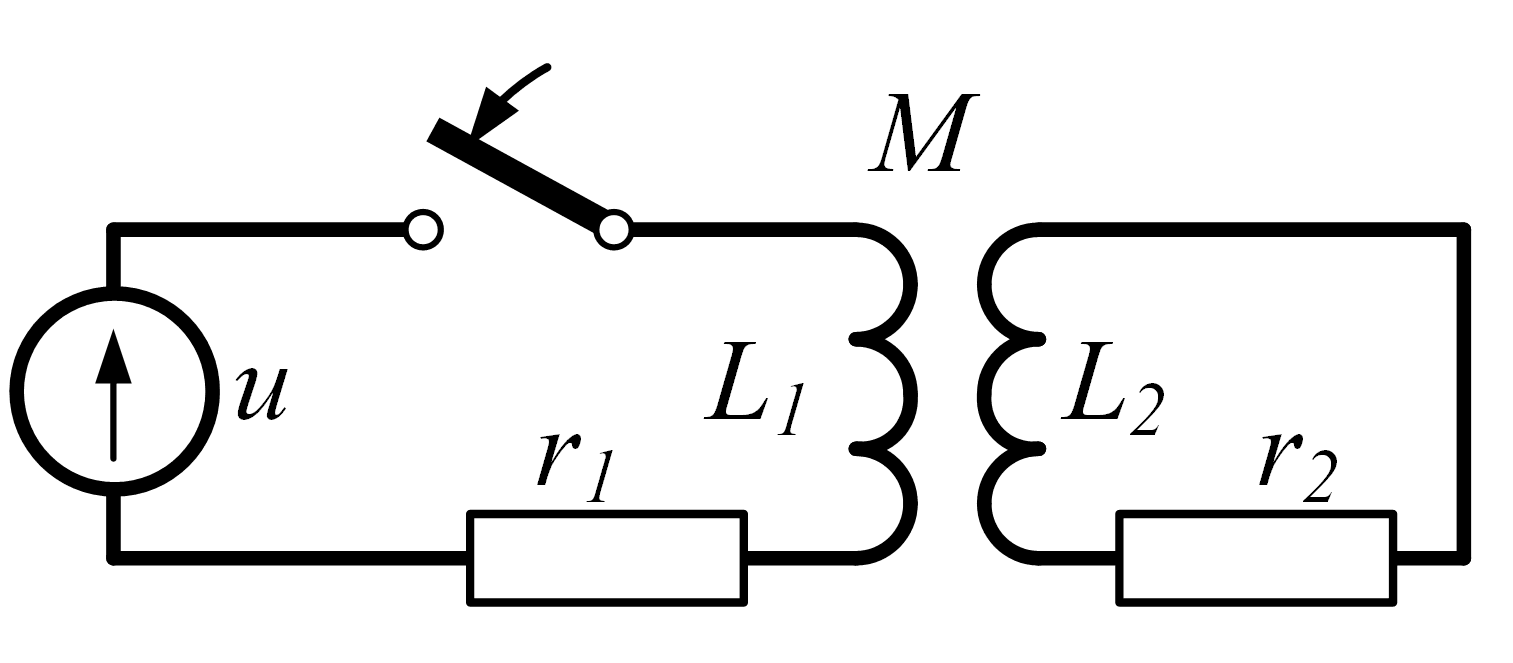
\includegraphics[width=0.40\linewidth]{pic/4-1}
	\caption{Простейшая цепь с магнитной связью.}
	\label{ris:4-1 simplest_circut}
\end{floatingfigure}

